\documentclass[11pt]{beamer}
\usepackage[utf8]{inputenc}
\usepackage[T1]{fontenc}
\usefonttheme[onlymath]{serif}
\usetheme{Frankfurt}
\usecolortheme{crane}
\author{Martin Averseng}
\usepackage{amsthm}
\title{\textbf{Parler de ma thèse à mes amis}\\}
\date{\today}
\makeatletter
\setbeamertemplate{headline}{%
	\begin{beamercolorbox}[ht=2.25ex,dp=3.75ex]{section in head/foot}
		\insertnavigation{\paperwidth}
	\end{beamercolorbox}%
}%
\makeatother
\AtBeginSection[]
{
	\begin{frame}<beamer>
		\tableofcontents[currentsection]
	\end{frame}
}
    \setbeamertemplate{frametitle}
    {\begin{centering}\smallskip
    		\insertframetitle\par
    		\smallskip\end{centering}}
    \setbeamertemplate{itemize item}{$\bullet$}
   \setbeamertemplate{navigation symbols}{}
    \setbeamertemplate{footline}[text line]{%
    	\hfill\strut{%
   		\scriptsize\sf\color{black!60}%
   		\quad\insertframenumber
   	}%
   	\hfill
    }
%    \theoremstyle{plain} % insert bellow all blocks you want in italic
\begin{document}
	\maketitle

	\section{Introduction}
	
	\begin{frame}
		\centering
		\begin{large}
			Introduction
		\end{large}
		\vspace{10pt}
		
		\begin{huge}
			Un bref historique des sciences
		\end{huge}	
	\end{frame}
	
	\begin{frame}
		\frametitle{La causalité}
		Parmi les événements que nous observons, beaucoup semblent inscrit dans une chaîne de cause et de conséquence.  
		
		Cette expérience de la causalité est omniprésente dans notre quotidien. Si je ne mange pas je meurs. Si je ne cours pas je serai en retard. Si je l'insulte, il sera énervé. 
		
		Y a-t-il une limite à tout ce que l'on peut prédire ? Certains événements sont-ils soumis aux caprices des dieux, ou de notre libre-arbitre ?  Si tout événement est la conséquence prévisible d'un autre comment peut-on prédire effectivement ? 
	\end{frame}
	
	
	\begin{frame}
		\frametitle{Prédire les mouvements des planètes}
		Dès l'antiquité, dans différents endroits du monde, l'homme sait prédire avec grande précision le mouvement des corps célestes. Les mayas étaient par exemple capables de prédire les jours d'éclipses de Vénus. \\
		
		Une logique semble à l'oeuvre derrière ces mouvements réguliers. \\
		% Photo de l'éclipse
		\begin{figure}
			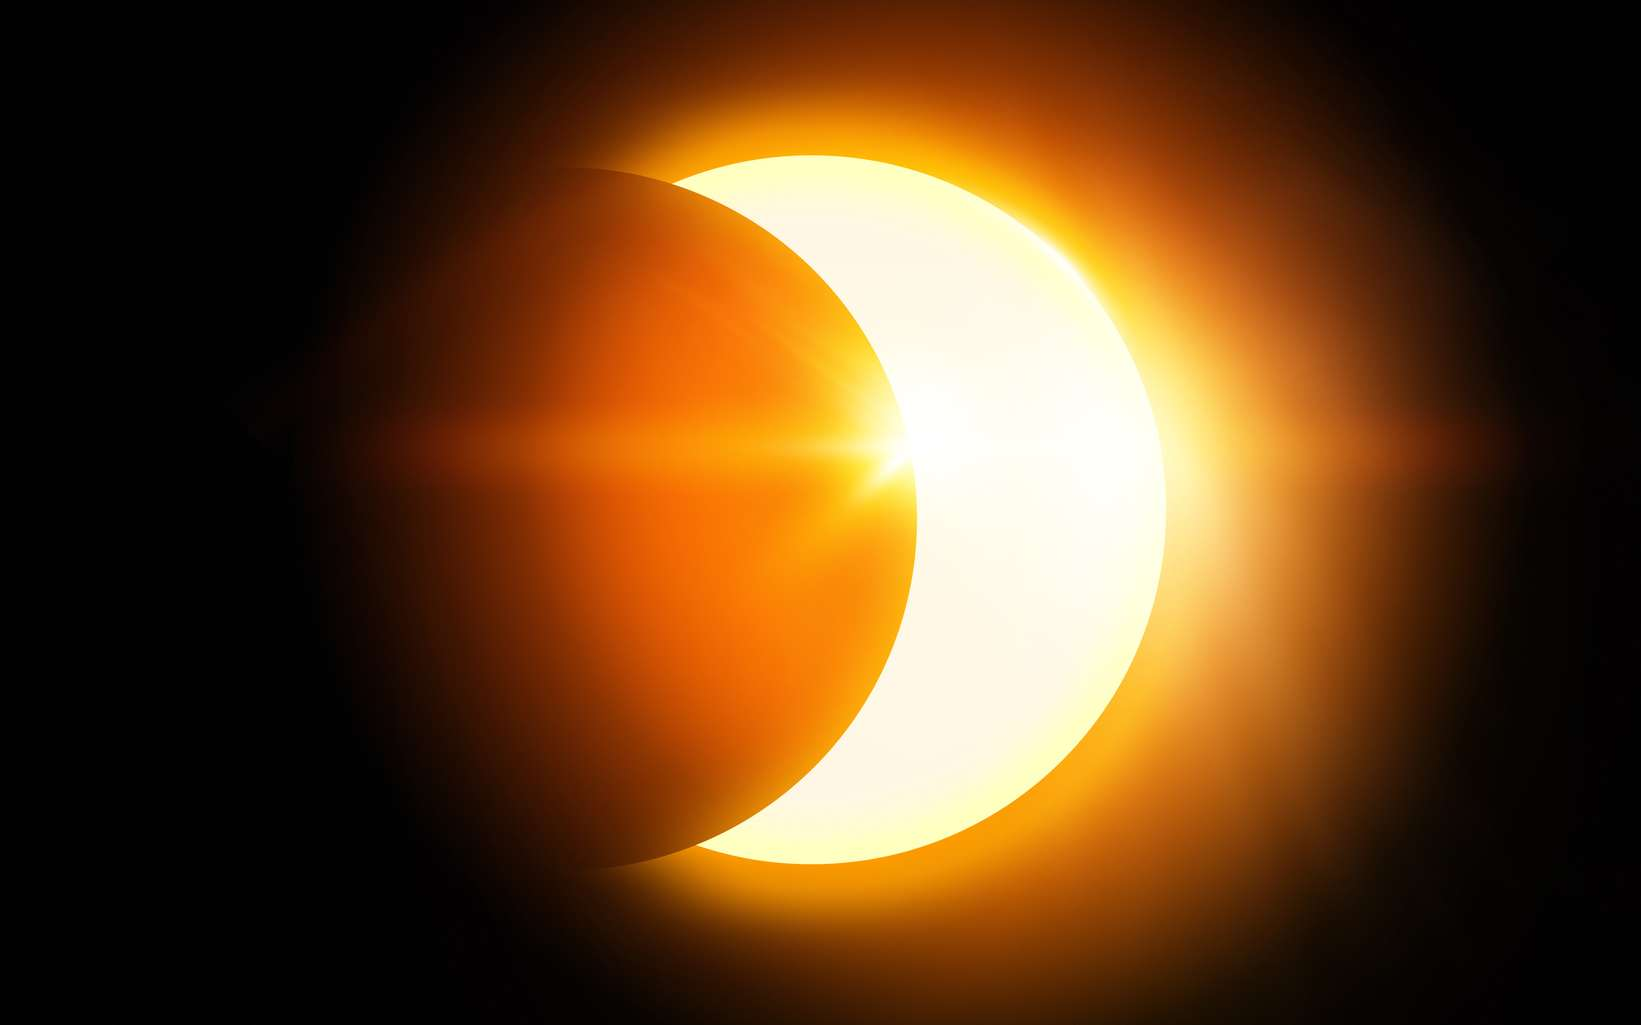
\includegraphics[scale=0.1]{eclipse}
		\end{figure}
	\end{frame}
	\begin{frame}
		\frametitle{Les lois de la nature}
		Au 17ème siècle, la prédiction du mouvement des planètes effectue un nouveau bond grâce à deux avancées de Newton. 
		
		\begin{itemize}
			\item[-] Les lois de Newton, qui permettent de prédire le déplacement d'un objet lorsqu'on connaît les \textbf{forces} qui lui sont appliquées
			\item[-] La loi de l'attraction universelle. Chaque corps exerce sur chaque autre corps de l'univers une \textbf{force} proportionnelle à sa masse et inversement proportionnelle au carré de la distance qui les sépare. 
		\end{itemize}
		\begin{figure}
			
\includegraphics[scale = 2]{newton}
		\end{figure}
	\end{frame}
	\begin{frame}
		\frametitle{Les lois de la nature}
		Les lois de la nature qu'on a formulé à partir du 17ème siècle ont les caractéristiques suivantes : 
		\begin{itemize}
			\item[-] Elles ne sont pas prouvées, ce ne sont que des hypothèses. 
			\item[-] Elles peuvent être approximative, c'es-à-dire qu'elles ne prédisent le futur qu'à une certaine erreur près (Domaine de validité).
			\item[-] Il n'existe pas (à ce jour) d'expérience reproductible qui puisse prouver que l'une d'entre elle est fausse dans son domaine de validité connu. 
			\item[-] Elles permettent de formuler des prédictions quantitatives précises sur le futur. 
			\item[-] Elles sont universelles : selon nos observations, tout objet de l'univers doit respecter ces lois. 
			\item[-] Elles sont inaltérables, ce qui signifie qu'il ne faut pas les modifer en fonction du contexte. 
		\end{itemize}
	\end{frame}
	\section{Les équations aux dérivées partielles}
	\begin{frame}\frametitle{Les lois de la physique}
		Les lois de la physique permettent de prédire l'évolution de grandeurs (pas forcément les déplacements d'un objets) dans le temps et l'espace. Par exemple, l'écoulement d'un fluide comme le sang dans le corps, l'évolution de la pression dans l'océan en fonction de la profondeur, l'oxydation d'un matériau, le champ électro-magnétique etc.
		
		
		Les équations aux dérivées partielles sont la forme commune à toutes les équations de la physique. Elles relient les "dérivées" de ces quantités (température, pression, vitesse, densité) par rapport au temps ou à des directions de l'espace, à des "forces", toujours selon le formalisme de Newton. 
		
		 
		
	\end{frame}
	\begin{frame}
		Des équations célèbres: 
		
	\end{frame}
		. 
	
	
	
	
	\setcounter{subsection}{1}
	\begin{frame}
		\frametitle{Methode BEM (Boundary Element Method)}
		Méthode de résolution numérique des EDP.
		\begin{minipage}{0.69\textwidth}
			Problème type : 
			\begin{equation*}
			\left\{
				\begin{aligned}
				-\Delta u &= 0 & \text{ dans } \Omega^e \text{ ou } \Omega^i\\
				u \text{ ou }\dfrac{\partial u}{\partial n} &= 0 & \text{ sur } \Gamma
				\end{aligned}
				\right.
			\end{equation*}
		\end{minipage}
		\begin{minipage}{0.29\textwidth}
			\begin{figure}
				\centering
			
			\end{figure}
		\end{minipage}
		\begin{minipage}{0.69\textwidth}
			Equations intégrales : inconnue = fonctions $\lambda$, $\mu$ définies sur la frontière $\Gamma$.\\
			Solution de l'équation dans $\Omega^{e,i}$ obtenue via représentation intégrale
			\[ u(x) = \int_{\Gamma}G(x,y) \lambda(y) -  \dfrac{\partial G}{\partial n_y}(x,y)\mu(y) dy, x \in \Omega\]
		\end{minipage}
		\begin{minipage}{0.29\textwidth}
		\begin{figure}
		\end{figure}
		\end{minipage}
	\end{frame}
	\begin{frame}
		\frametitle{Caractéristiques de la méthode}
		\textbf{Deux classes de méthodes}
		\begin{itemize}
			\item Collocation (peu de résultats de convergence)
			\item \textbf{Galerkine} (cadre Sobolev, doubles intégrales)
		\end{itemize}
		\textbf{Avantages principaux :}
		\begin{itemize}
			\item Domaines infinis
			\item Maillages plus simples 
			\item Excellente précision 
		\end{itemize}
		\textbf{Difficultés majeures :}
		\begin{itemize}
			\item Evaluation numérique d'intégrales singulières
			\item Systèmes linéaires denses
			\item Connaissance requise d'une solution fondamentale
		\end{itemize}
		
	\end{frame}
	\begin{frame}
		\frametitle{Applications industrielles}
		
		\textbf{Acoustique} : problèmes de diffraction, simulation de la propagation du son dans une cavité et recherche de modes (habitacles de voitures / avions, radar / sonar). \\
		\textbf{Elasticité} : Vérification des matériaux, critère de fracture (application en excavation par exemple.)
		\begin{figure}
			\centering
			\caption{Les trois modes de fracture}
		\end{figure}
		Mais aussi électromagnétisme, écoulements irrotationnels, traitement d'image, systèmes de particules...\\
		\textbf{Problèmes inverses} : méthodes itératives. 		
	\end{frame}
	
	\section{Représentation intégrale}
	\setcounter{subsection}{1}
	\begin{frame}
		\frametitle{Modèle d'EDP}
		\begin{block}{Classe d'EDP :}			
			\[\mathcal{P}u = - \text{div}(A \nabla u) + b\cdot \nabla u + c u\]
		\end{block}		
		Avec la condition d'ellipticité : A définie positive. 
		\begin{block}{Definition}
			Dérivée conormale sur $\Gamma$ :
			\[ \mathcal{B}_\nu u(y) := \left(A\nabla u(y)\right) \cdot \nu(y).\]
		\end{block}
		Pour le Laplacien, $\mathcal{B}_\nu \equiv$ dérivée normale. 
		Généralisations : coefficients non constants, EDP vectorielles, $A$ complexe et pas nécessairement en forme divergence. 		
	\end{frame}
	\begin{frame}
		\frametitle{Solution fondamentale}
		Un opérateur linéaire $\mathcal{G}$ est appelé une solution fondamentale pour $\mathcal{P}$ si
		\[\mathcal{P}\mathcal{G}u = u = \mathcal{P}\mathcal{G}u,\]
		avec $\mathcal{G}$ de la forme 
		\[ \mathcal{G}u(x) = \int_{\mathbb{R}^n} G(x,y) u(y) dy\]
		On appelle $G(x,y) = G(x-y)$ le noyau de Green de l'opérateur, et on a 
		\[ \mathcal{P}G = \delta\]
		(Attention : Pas d'unicité pour $G$). 
	\end{frame}
	\begin{frame}
		\frametitle{Condition de radiation}
		$B_\rho$ une boule qui contient (compactement) $\Omega^i$. 
		\[\mathcal{M}u(x) := \int_{\partial B_\rho} G(x,y) \mathcal{B}_\nu u(y) - \mathcal{B}_{\nu,y}G(x,y)u(y)d\sigma(y) \]
		\begin{block}{Lemme}
			Si $\mathcal{P}u = 0$ dans $\Omega_e$, $\mathcal{M}$ ne dépend pas du choix de $\rho$. 
		\end{block}
		Condition de radiation dépend de la solution fondamentale $G$ : 
		\[ \mathcal{M}u = 0 \quad \text{ identiquement sur } \mathbb{R}^n.\] 
		\vspace{-0.5cm}
		\begin{itemize}
			\item $\mathcal{P} = \text{div}(B \nabla u)$ : Condition de radiation équivaut à condition de décroissance à l'infini sur $u(x)$ et $B_\nu u(x)$. 
			\item Equation de Helmholtz $\mathcal{P}u = -\Delta u - k^2 u$ : condition de radiation de Sommerfeld 
			\[ \lim_{\rho \to \infty} \rho^{(n-1)/2} \left(\frac{\partial u}{\partial \rho} - iku \right) = 0\]
		\end{itemize}
	
	\end{frame}
	\begin{frame}
		\frametitle{Réprésentation intégrale pour l'équation de Laplace.}
		Noyau de Green : 
		\[G(z) = \begin{cases}
		- \frac{1}{2\pi} \log |z| & \text{ en dimension } 2\\
		 \frac{1}{4\pi|z|} & \text{ en dimension } 3
		\end{cases}\]\\
		On note $\left[\phi\right] = \gamma^+ \phi - \gamma^- \phi$ saut d'une distribution $\phi$ à travers $\Gamma$. 
		\begin{block}{Théorème}
			Si $u\in H^1_{loc}(\Omega^{i,e})$, vérifie la condition de radiation, $\Delta u = 0$ sur $\Omega^i$ et $\Omega^e$, alors $\forall x \notin \Gamma$
			\[u(x) = \int_{\Gamma}G(x,y)\left[\dfrac{\partial{u}}{\partial \nu_y}\right](y) - \dfrac{\partial G}{\partial \nu_y}(x,y)\left[u\right](y) dy  \]
		\end{block}
		
	\end{frame}
	\begin{frame}{Plus généralement}
		\begin{block}{Théorème}
			Soit $u$ défini par $u_{i}$ sur $\Omega^i$ et $u_e$  sur $\Omega^e$ tel que 
			\[\mathcal{P}u_{i,e} = 0, \quad \text{sur } \Omega_{i,e}\] 
			Alors, pour $x\notin \Gamma$, 
			\[u(x) = \int_{\Gamma} G(x,y) \left[\mathcal{B}_\nu u\right](y)- \mathcal{B}_{\nu,y}G(x,y) \left[u\right](y) d\sigma(y) \] 
		\end{block}
		
		\begin{Definition}
			Potentiel de simple couche : $\mathcal{S} \lambda := \int_{\Gamma} G(x,y) \lambda(y) d\sigma(y)$\\
			Potentiel de double couche : $\mathcal{D} \mu := \int_{\Gamma} {\mathcal{B}}_{\nu,y}G(x,y) \mu(y) d\sigma(y)$
		\end{Definition} 
	\end{frame}
	\section{Projecteurs de Calderòn}
	\setcounter{subsection}{1}
	\begin{frame}
		\frametitle{Relations de saut}
		Pour tout fonction $u$ telle que $\mathcal{P}u = 0$ sur $\Omega^{i,e}$, on a, en notant $\lambda$ et $\mu$ les sauts de $u$ et de sa dérivée normale:
		\[ u(x) = \mathcal{S}\lambda(x) - \mathcal{D}\mu(x) \in C^{\infty}(\Omega^{i,e}).\]
		Pour aboutir à une équation intégrale, on fait tendre $x$ vers un point de $\Gamma$, par l'intérieur ou l'extérieur.
		\alert{Il ne suffit pas de passer à la limite sous l'intégrale} : 
		\begin{block}{Relations de saut}
			On a les relations suivantes :
			\vspace{-0.4cm}
			\begin{eqnarray*}
			\left[\mathcal{S}\lambda\right] &=& 0\\
			\left[\mathcal{B}_\nu\mathcal{S}\lambda\right] &=& \lambda\\
			\left[\mathcal{D}\mu\right] &=& -\mu\\
			\left[\mathcal{B}_\nu\mathcal{D}\mu\right] &=& 0
			\end{eqnarray*}
		\end{block}
	\end{frame}
	\begin{frame}
		\frametitle{Traces des potentiels $\mathcal{S}$ et $\mathcal{D}$}
	    On pose $S = \gamma \mathcal{S}$, $D = \left(\gamma^+ + \gamma^-\right)\mathcal{D}$, $T = \frac{1}{2}(\mathcal{B}_\nu^+ +  \mathcal{B}_\nu^- )\mathcal{S}$, $R = -\mathcal{B}_\nu\mathcal{D}$. En fait, $T = D^*$. 
		\begin{block}{Représentation intégrale des opérateurs surfaciques}
			\[S\lambda(x) = \int_{\Gamma} G(x,y) \lambda(y) d\sigma(y)\]
			Lorsque $\Gamma$ possède un plan tangent au point $x$, 
			\[D\mu(x) = \int_{\Gamma}\mathcal{B}_{\nu,y} G(x,y) \mu(y)d\sigma(y)\]
			Si $\Gamma$ est de classe $C^2$ au voisinnage de $x$, 
			\[R\mu(x) = \text{p.f.} \int_{\Gamma\setminus{B_\varepsilon}(x)}B_{\nu,x}B_{\nu,y}G(x,y) \mu(y) dy \]
		\end{block}
		Le dernier opérateur a un noyau qualifié d'"hyper-singulier". 
	\end{frame}
	\begin{frame}
		\frametitle{Continuité dans les espaces de Sobolev}
		L'étude de la continuité de $S$, $D$ et $R$ dans les espaces de Sobolev a fait l'objet de beaucoup d'efforts dans les 50 dernières années. 
		$H^s(\Gamma)$ espaces de Sobolev définit sur la frontière d'un ouvert.  
		\begin{block}{Théorème}
			Pour tout $-\frac{1}{2} \leq s \leq \frac{1}{2}$ les applications linéaires suivantes sont continues:
			\vspace{-0.4cm}
			\begin{eqnarray*}
				S &:& H^{s-1/2}(\Gamma) \to H^{s+1/2}(\Gamma)\\
				D &:& H^{s+1/2}(\Gamma) \to H^{s+1/2}(\Gamma)\\
				D^*&:& H^{s-1/2}(\Gamma) \to H^{s-1/2}(\Gamma)\\
				R &:& H^{s+1/2}(\Gamma) \to H^{s-1/2}(\Gamma)
			\end{eqnarray*}
		\end{block}	
		Cas d'égalité notoirement difficiles lorsque $\Gamma$ n'est que Lipschitz. Propriété de Fredholm héritée de la coercivité de $\mathcal{P}$. 	
	\end{frame}
	\begin{frame}
		Influence de la régularité du domaine
		\begin{block}{Théorème}
			Lorsque $\Gamma$ est de classe $C^{1+\mu}$, pour un certain $0<\mu < 1$, $D$ est continu de $L^{\infty}(\Gamma)$ dans $C^{\mu}(\Gamma)$. $D$ est compact de $C^\lambda(\Gamma)$ dans lui-même pour $0\leq \lambda \leq \mu$. 
		\end{block}
		Lorsque $\Gamma$ a un "coin", $D$ n'est plus compact.
		La régularité du domaine est un point épineux de la théorie et le centre du sujet de ma thèse. Polygônes, écrans. 
	\end{frame}
	\begin{frame}
		\frametitle{Calcul numérique de $S$, $D$ et $R$}
		C'est l'un des aspects critiques de la méthode !
		\begin{itemize}
			\item Lorsque $x$ et $y$ sont éloignés : quadrature numérique.
			\item Lorsque $x$ et $y$ sont prohches : deux options : formules exactes pour des fonctions tests simples (polynômes par morceaux) ou changements de coordonnées pour retirer la singularité. 
		\end{itemize}
		Pour le noyau hyper-singulier, méthode par intégration par parties. Dans le cas de l'équation de Laplace, par exemple
		\[(R\phi,\psi) = (S \overrightarrow{\text{rot}}_\Gamma \phi, \overrightarrow{\text{rot}}_\Gamma\psi)\]
		Où $\overrightarrow{\text{rot}}_\Gamma$ est le rotationnel surfacique sur $\Gamma$... (abscisse curviligne en 2D)
	\end{frame}
	\begin{frame}
		\frametitle{Projecteurs de Calderòn}
		Pour tout $\lambda, \mu$, en posant $u = \mathcal{S}\lambda - \mathcal{D}\mu$
		\begin{equation*}
			\begin{pmatrix}
			u^i  \\
			\mathcal{B}_\nu u^i
			\end{pmatrix} = 
			\begin{pmatrix}
			\frac{I}{2} - D & S \\
			-R & \frac{I}{2} + D^*
			\end{pmatrix}
			\begin{pmatrix}
			\lambda  \\
			\mu
			\end{pmatrix}
		\end{equation*}
		\begin{equation*}
		\begin{pmatrix}
		u^e  \\
		\mathcal{B}_\nu u^e
		\end{pmatrix} = 
		\begin{pmatrix}
		-\frac{I}{2} - D & S \\
		-R & -\frac{I}{2} + D^*
		\end{pmatrix}
		\begin{pmatrix}
		\lambda  \\
		\mu
		\end{pmatrix}
		\end{equation*}
		$C_i := \begin{pmatrix}
		\frac{I}{2} - D & S \\
		-R & \frac{I}{2} + D^*
		\end{pmatrix}$, 
		$C_e:=\begin{pmatrix}
			\frac{I}{2} - D & S \\
			-R & \frac{I}{2} + D^*
		\end{pmatrix} = I - C_i$ projecteurs. 
		\begin{block}{Relations de Calderòn}
			\centering
			$DS = SD^*$, $RD = D^*R$, $SR = \frac{I}{4} - D^2$, $RS = \frac{I}{4} - D^{*2}$
		\end{block}
	\end{frame}
	\begin{frame}
		\frametitle{Equations intégrales}
		Reformulation d'un problème aux limites en termes des opérateurs $S$, $D$ et $R$. 
		Exemple : problème de Dirichlet intérieur pour le Laplacien. 
		\begin{block}{Théorème}
			Soit $g$ une fonction régulière définie sur $\Gamma$. Si $u_i \in H^1(\Omega^i)$ est une solution de 
			\[\left\{ \begin{array}{ccl}
			-\Delta u_i &= 0 &\text{ dans } \Omega^i\\
			\gamma u_i &= g & \text{ sur }\Gamma 
			\end{array}\right.\]
			alors $\psi:=\mathcal{B}_\nu^- u_i$ est une solution de l'équation intégrale 
			\[S\psi = \left(\frac{I}{2}+D\right)g\]
			Réciproquement si $\psi$ est une solution de l'équation intégrale,  $-\mathcal{S}\psi + \mathcal{D}g$ définit une solution du problème de Dirichlet intérieur. 
		\end{block}
	\end{frame}
		\begin{frame}
			\frametitle{Problèmes d'unicité}
			Il peut arriver que l'équation intégrale qu'on a formulée n'ait pas une unique solution, malgré le fait que ce soit le cas pour le problème de départ.
			\begin{block}{Théorème}
				Soit $\mathcal{P} = -\Delta u - k^2u$ l'opérateur de Helmholtz. Le problème de Dirichlet extérieur pour $\mathcal{P}$ (+ condition de Sommerfeld) admet une solution unique pour toute donnée $g \in H^{1/2}(\Gamma)$. 
			\end{block}
			mais pourtant,
			\begin{block}{Théorème}
				$\text{Ker }S = \{0\} \Leftrightarrow k^2$ n'est pas une valeur propre intérieure du Laplacien.   
			\end{block}
			En pratique : induit des problèmes de conditionnement de l'opérateur intégral lorsque $k^2$ est proche d'une valeur propre. Astuce de Brackage-Werner. 
		\end{frame}
	\section{Eléments finis de frontière}
	\setcounter{subsection}{1}
	\begin{frame}
		\frametitle{Etude d'un problème type}
		On va étudier le cas $\mathcal{P} = - \Delta$, et le problème de Dirichlet extérieur en dimension $3$. 
		\[\left\{ \begin{array}{rll}
		\Delta u &= 0 &\text{ dans } \Omega^e\\
		u &= g &\text{ sur } \Gamma\\
		|u(x)| &= O(\frac{1}{|x|})& \text{ à l'infini} 
		\end{array}\right.\]
		\begin{block}{Théorème}
			Cette équation a une unique solution dans $H^1_{\text{loc}}(\Omega^e)$. 
		\end{block}
		On utilise la reformulation par équation intégrale 
		\[S\lambda = b := \left(\frac{I}{2} + D\right)g\]
	\end{frame}
	\begin{frame}
		\frametitle{Formulation variationnelle}
		On utilise une formulation de type Galerkine de l'équation intégrale, à savoir 
		\[\left( S\lambda| \mu \right)_{\Gamma} = (b,\mu)_{\Gamma}.\]
		C'est-à-dire, 
		\[\int_{\Gamma}\int_{\Gamma}\dfrac{\lambda(x) \mu(y)}{4\pi|x - y|} dxdy = \int_{\Gamma} b(y) \mu(y) dy\]
		La forme bilinéaire est coercive. Espace variationnel $V_h \subset H^{-1/2}(\Gamma)$ de dimension finie. 
		Solution approchée : $\varphi_h \in V_h$ telle que
		\[\left( S\lambda_h| \mu \right)_{\Gamma} = (b,\mu)_{\Gamma} \text{ pour tout } \mu \in V_h\]
		Lemme de Céa du à la forte ellipticité de la forme bilinéaire. 
		\begin{block}{Théorème}
			\[ || \varphi - \varphi_h|| \leq C \inf_{\mu \in V_h}||\varphi - \mu||\]
		\end{block} 	
	\end{frame}
	\begin{frame}
		\frametitle{Inégalité de Garding, optimalité asymptotique}
		Remarque avant de donner la vitesse de convergence :\\
		Pour un opérateur $\mathcal{P}$ général (par exemple Helmholtz, Maxwell etc.), $S$ et $R$ ne sont pas nécessairement fortement elliptiques. On a en revanche toujours l'inégalité de Garding suivante : 
		\begin{Theorem}
			Il existe deux opérateurs compacts $L_1 : H^{-1/2}(\Gamma) \to H^{1/2}(\Gamma)$ et $L_2 : H^{1/2}(\Gamma) \to H^{-1/2}(\Gamma)$ tels que
			\[(\phi,(S + L_1)\phi) \geq c||\phi||_{H^{-1/2}(\Gamma)}^2\] 
			\[(\phi,(R + L_2)\phi) \geq c||\phi||_{H^{1/2}(\Gamma)}^2\] 
		\end{Theorem} 
	\end{frame}
	\begin{frame}
		\frametitle{Inégalité de Garding, quasi-optimalité asymptotique}
		L'inégalité de Garding suffit à garantir la quasi-optimalité pour un maillage assez fin. 
		\begin{Theorem}
			Si la famille $E_h$ est "dense" dans $E$, si $b$ est une forme bilinéaire sur $E$ satisfaisant une inégalité de Garding, et si le problème 
			\[b(u,v) = l(v)\]
			possède une unique solution $u$, alors pour un certain $h_0$, le problème variationnel discret a une unique solution pour tout $h < h_0$. 
		\end{Theorem}
	\end{frame}
	\begin{frame}
		\frametitle{Vitesse de convergence pour des fonctions constantes par morceaux}
		On considère $V_h$ l'espace des fonctions constantes par morceaux sur un maillage suffisamment "uniforme" (je n'ai pas envie de préciser)
		\begin{block}{Théorème}
			On suppose que la solution exacte est dans $H^s(\Gamma)$, $0 \leq s \leq 1$. 
			\[|| \varphi - \varphi_h||_{H^{-1/2}(\Gamma)} \leq C h^{s+1/2}||\varphi||_{H^s(\Gamma)}\]
		\end{block}
		Lorsque la solution est régulière, la solution approchée converge plus vite vers la solution exacte (même situation que les éléments finis). 
		
	\end{frame}
	\begin{frame}\frametitle{Vitesse de convergence en présence de coins}
		Lorsque le domaine comporte des singularités géométriques, la solution n'est pas régulière $\to$ étude asymptotique combinée avec l'une des méthodes suivantes : 
		\begin{itemize}
			\item[-] Raffinement du maillage / augmentation de l'ordre polynomial / un mélange des deux (méthodes hp)
			\item[-] Espaces de fonctions "augmentés" (on inclut dans $V_h$ une fonction ayant la bonne asymptotique au coin. 
			\item[-] (Un de mes axes de recherche) Changement de variable. 
		\end{itemize}
	\end{frame}
	
	\section{Résolution numérique}
	\setcounter{subsection}{1}
	\begin{frame}
		Une fois que la formulation variationelle a été discrétisée, on est ramené à la résolution d'un système linéaire $N \times N$.  
		\[Bu = L\]
		Où $B_{i,j} = \int_{\Gamma\times\Gamma} G(x-y) \phi_i(x) \phi_j(y)$ (pleine !)
		Et où $u$ est le vecteur des coordonnées de la solution approchée dans la base des fonctions $\phi_i$. 
		En général : méthodes itératives. Deux difficultés majeures. 
		\begin{itemize}
			\item[-] Compression et accélération du produit matrice vecteur.
			\item[-] Préconditionnement du système linéaire : centre du sujet de ma thèse. 
		\end{itemize}
	\end{frame}
	\begin{frame}
		\frametitle{Quelques mots sur les méthodes d'accélération compression}
		FMM méthode la plus utilisée actuellement. Réduit la complexité du produit matrice-vecteur de $N^2$ à $Nlog(N)$. 
		Deux défauts : 
		\begin{itemize}
			\item TRES compliqué (illustration : cours sur la FMM)
			\item Formules différentes pour chaque noyau $G$ (développements asymptotiques)
		\end{itemize}
		Méthode SCSD : développée par Matthieu Aussal (pendant sa thèse) et François Alouges au CMAP. Méthode très intuitive (j'explique au tableau). 
		Mon dernier papier : version 2D de la SCSD (qui n'était que disponible en 3D) avec estimation de complexités. 
	\end{frame}
	\begin{frame}
		\frametitle{Quelques mots sur le préconditionnement}
		\begin{itemize}
			\item Préconditionnement "de Calderòn", mais on préférerait des préconditionneurs locaux !
			\item Approches pseudo-différentielles, mais tout s'écroule quand le domaine a des coins. 
		\end{itemize}
	\end{frame}
\end{document}